\documentclass[11pt,letter]{article}
\usepackage{etex}
\usepackage[top=0.65in,bottom=0.9in,left=0.85in,right=0.85in]{geometry}

%\def\baselinestretch{1.25}
\def\baselinestretch{1.0}

\usepackage[greek, english]{babel}
%\usepackage{multicol}
\usepackage[thinlines]{easytable}

%\usepackage[draft]{graphicx}
\usepackage{graphicx}
\usepackage[export]{adjustbox}

\usepackage{caption}
\usepackage{subcaption}

\usepackage{setspace}
\usepackage{float}

% The use of the times package forces the use of the type-1 times
% roman font, but the times roman font does not look nice.
% Besides the times roman font still does not print correctly on
% the dopy printer.
%\usepackage{times}


\usepackage{fancyhdr}
\usepackage{amsmath}
\usepackage{amssymb}
\usepackage{bm}
\usepackage{bbold}
\usepackage{parskip}
\usepackage{url}

\newcommand{\kb}{\ensuremath{k_{\text{B}}}}

\newcommand{\bv}[1]{\ensuremath{\bm{#1}}}
\newcommand{\Lc}{\ensuremath{L_{\mathrm{c}}}}
\newcommand{\dsig}[1]{\ensuremath{ \frac{ d\,\sigma_{#1} }{d\,\Omega} }}

\newcommand{\isat}{\ensuremath{I_{\mathrm{sat}}}}
\newcommand{\iisat}{\ensuremath{I_{\mathrm{p}}/I_{\mathrm{sat}}}}
\newcommand{\Iqtof}{\ensuremath{I_{\bv{Q}\infty} }}
\newcommand{\Itof}[1]{\ensuremath{I_{\bv{#1}\infty} }}
\newcommand{\Iq}{\ensuremath{I_{\bv{Q}} }}
\newcommand{\iq}{\ensuremath{i_{\bv{Q}} }}
\newcommand{\Iqma}{\ensuremath{I_{\bv{Q}_{\text{MA}}} }}
\newcommand{\Ima}[1]{\ensuremath{I_{\bv{#1}_{\text{MA}}} }}
\newcommand{\iqma}{\ensuremath{i_{\bv{Q}_{\text{MA}}} }}
\newcommand{\jqma}{\ensuremath{j_{\bv{Q}_{\text{MA}}} }}
\newcommand{\Iqmatof}{\ensuremath{I_{\bv{Q}_{\text{MA}\infty}} }}
\newcommand{\is}{\ensuremath{i_{S}} }
\newcommand{\iqT}{\ensuremath{i_{\bv{Q}_{T}} }}
\newcommand{\ipith}{\ensuremath{i_{\bv{\pi}/\bv{\theta}}}}
\newcommand{\fpith}{\ensuremath{f_{\bv{\pi}/\bv{\theta}}}}
\newcommand{\iT}[1]{\ensuremath{i_{\bv{#1}_{T}} }}
\newcommand{\ima}[1]{\ensuremath{i_{\bv{#1}_{\text{MA}}} }}
\newcommand{\fma}[1]{\ensuremath{f_{\bv{#1}_{\text{MA}}} }}
\newcommand{\jma}[1]{\ensuremath{j_{\bv{#1}_{\text{MA}}} }}

\newcommand{\pin}{\ensuremath{ P_{\text{i}}} }
\newcommand{\pret}{\ensuremath{ P_{\text{r}}} }
\newcommand{\win}{\ensuremath{ w_{\text{in}}} }
\newcommand{\wret}{\ensuremath{ w_{\text{r}}} }
\newcommand{\wir}{\ensuremath{ w_{\text{ir}}} }

\newcommand{\pgr}{\ensuremath{ P_{\text{gr}}} }
\newcommand{\wgr}{\ensuremath{ w_{\text{gr}}} }

\newcommand{\dbl}{\ensuremath{ \!\uparrow\! \downarrow \, }}
\newcommand{\spup}{\ensuremath{ \!\uparrow }}
\newcommand{\spdn}{\ensuremath{ \!\downarrow}}

\newcommand{\rdiag}{\ensuremath{ r_{\text{\tiny{111}}} } }
\newcommand{\awaist}{\ensuremath{ \alpha_{w} }}  
\newcommand{\awaistevap}{\ensuremath{ \alpha_{w,\text{evap}} }}  

\begin{document}


\section{ Spin structure factor }

Our experiment measures the bulk spin structure factor $\bar{S}_{\bv{Q}}$ for
an inhomogeneous realization of the Hubbard model.  Theoretical approaches such
as QMC and NLCE consider a homogenous system with a finite number of lattice
sites $L^{3}$ and  calculate the structure factor 
\begin{equation} 
    S_{\bv{Q}} = \frac{4}{L^{3}} \sum_{i,j} 
     e^{i\bv{Q}\cdot ( \bv{R}_{i} - \bv{R}_{j} )} \langle \sigma_{zi} \sigma_{zj}  \rangle
\end{equation}

In the local density approximation we can think of every point $\bv{r}$ of our
lattice site as a homogeneous system for which $S_{\bv{Q}}(\bv{r})$ can be
obtained.  We can relate the measured bulk spin structure factor
$\bar{S}_{\bv{Q}}$ to the local $S_{\bv{Q}}(\bv{r})$ as
\begin{equation}
  \bar{S}_{\bv{Q}}  = \frac{1}{N} \int  S_{\bv{Q}}(\bv{r}) \, \mathrm{d}^{3} \bv{r}
\end{equation}

The NLCE data provided by Ehsan gives $S_{\bv{Q}}$ directly whereas the QMC
data provided by Thereza gives $S_{\bv{Q}}/n$.  To compare with experiment we
have decided to use $S_{\bv{Q}}/n$ such that  
\begin{equation}
  \bar{S}_{\bv{Q}}  = \frac{1}{N} 
   \int \left[ \frac{  S_{\bv{Q}} }{n} \right]_{\bv{r}}
    n(\bv{r})  \, \mathrm{d}^{3} \bv{r}
\end{equation}

Also, in our LDA calculations we have assumed that there is spherical symmetry
in the system so 
\begin{equation}
  \bar{S}_{\bv{Q}}  = \frac{4\pi}{N} 
   \int \left[ \frac{  S_{\bv{Q}} }{n} \right]_{r_{d}}
    n(r_{d}) \,\, r_{d}^{2}   \, \mathrm{d}r_{d}
\end{equation}
where $r_{d}$ is the distance from the origin along a 111 body diagonal of the
lattice.  This last point can generate significant discussion since  away from
the diagonal the lattice depths are different along the $x,y,z$ directions and
an anisotropic Hubbard model should be used. However, for simplicity this is
how we decided to treat the system. 

\section{ NLCE data }

Ehsan has provided us with exact NLCE (numerical linked-cluster expansion) data
down to $T/t=1.6$.  Below this temperature he can do a resummation to obtain
the thermodynamic quatities.  At values of the temperature around $T/t=0.4$ the
results start getting very noisy, however we can recover a useable data set by
applying a low pass filter to the data\footnote{The type of filter used is the
Savitzky-Golay filter
\url{http://www.wire.tu-bs.de/OLDWEB/mameyer/cmr/savgol.pdf}}.  The original
data and the filtered data are shown in Fig.~\ref{fig:NLCE_T0.40}.  Larger
$T/t$ values are less noisy, but the filter is still used up to $T/t=1.4$ to
remove some spurious points that show up in the data.  At $T/t > 1.6$ the data
is exact and it has no spurious points.

%\begin{figure}
%        \centering
%        \begin{subfigure}[t]{0.4\textwidth}
%		\includegraphics[width=\textwidth]{figures/bands1d_V0_firstquant.png}
%\caption{ Band structure when the zero of energy is at the bottom of the
%lattice sites.  The zero of energy does not change with lattice depth, and the
%band energies go up almost like the harmonic oscillator state in an individual
%lattice site.  }
%                \label{fig:Hubbard-firstquant}
%        \end{subfigure}%
%        ~~ %add desired spacing between images, e. g. ~, \quad, \qquad etc.
%          %(or a blank line to force the subfigure onto a new line)
%        \begin{subfigure}[t]{0.4\textwidth}
%		\includegraphics[width=\textwidth]{figures/bands1d_V0_secondquant.png}
%\caption{ Band structure when the zero of energy is at the center of the lowest
%band.  This shift is implicit when the hamiltonian is written in second
%quantized form as in Eq.~\ref{eq:Hubbard-free-secondquant}.  }
%                \label{fig:Hubbard-secondquant}
%        \end{subfigure}
%	\caption{ Band structure in the Hubbard model.  }
%\label{fig:Hubbard-first-second}
%\end{figure}

\begin{figure}
    \centering
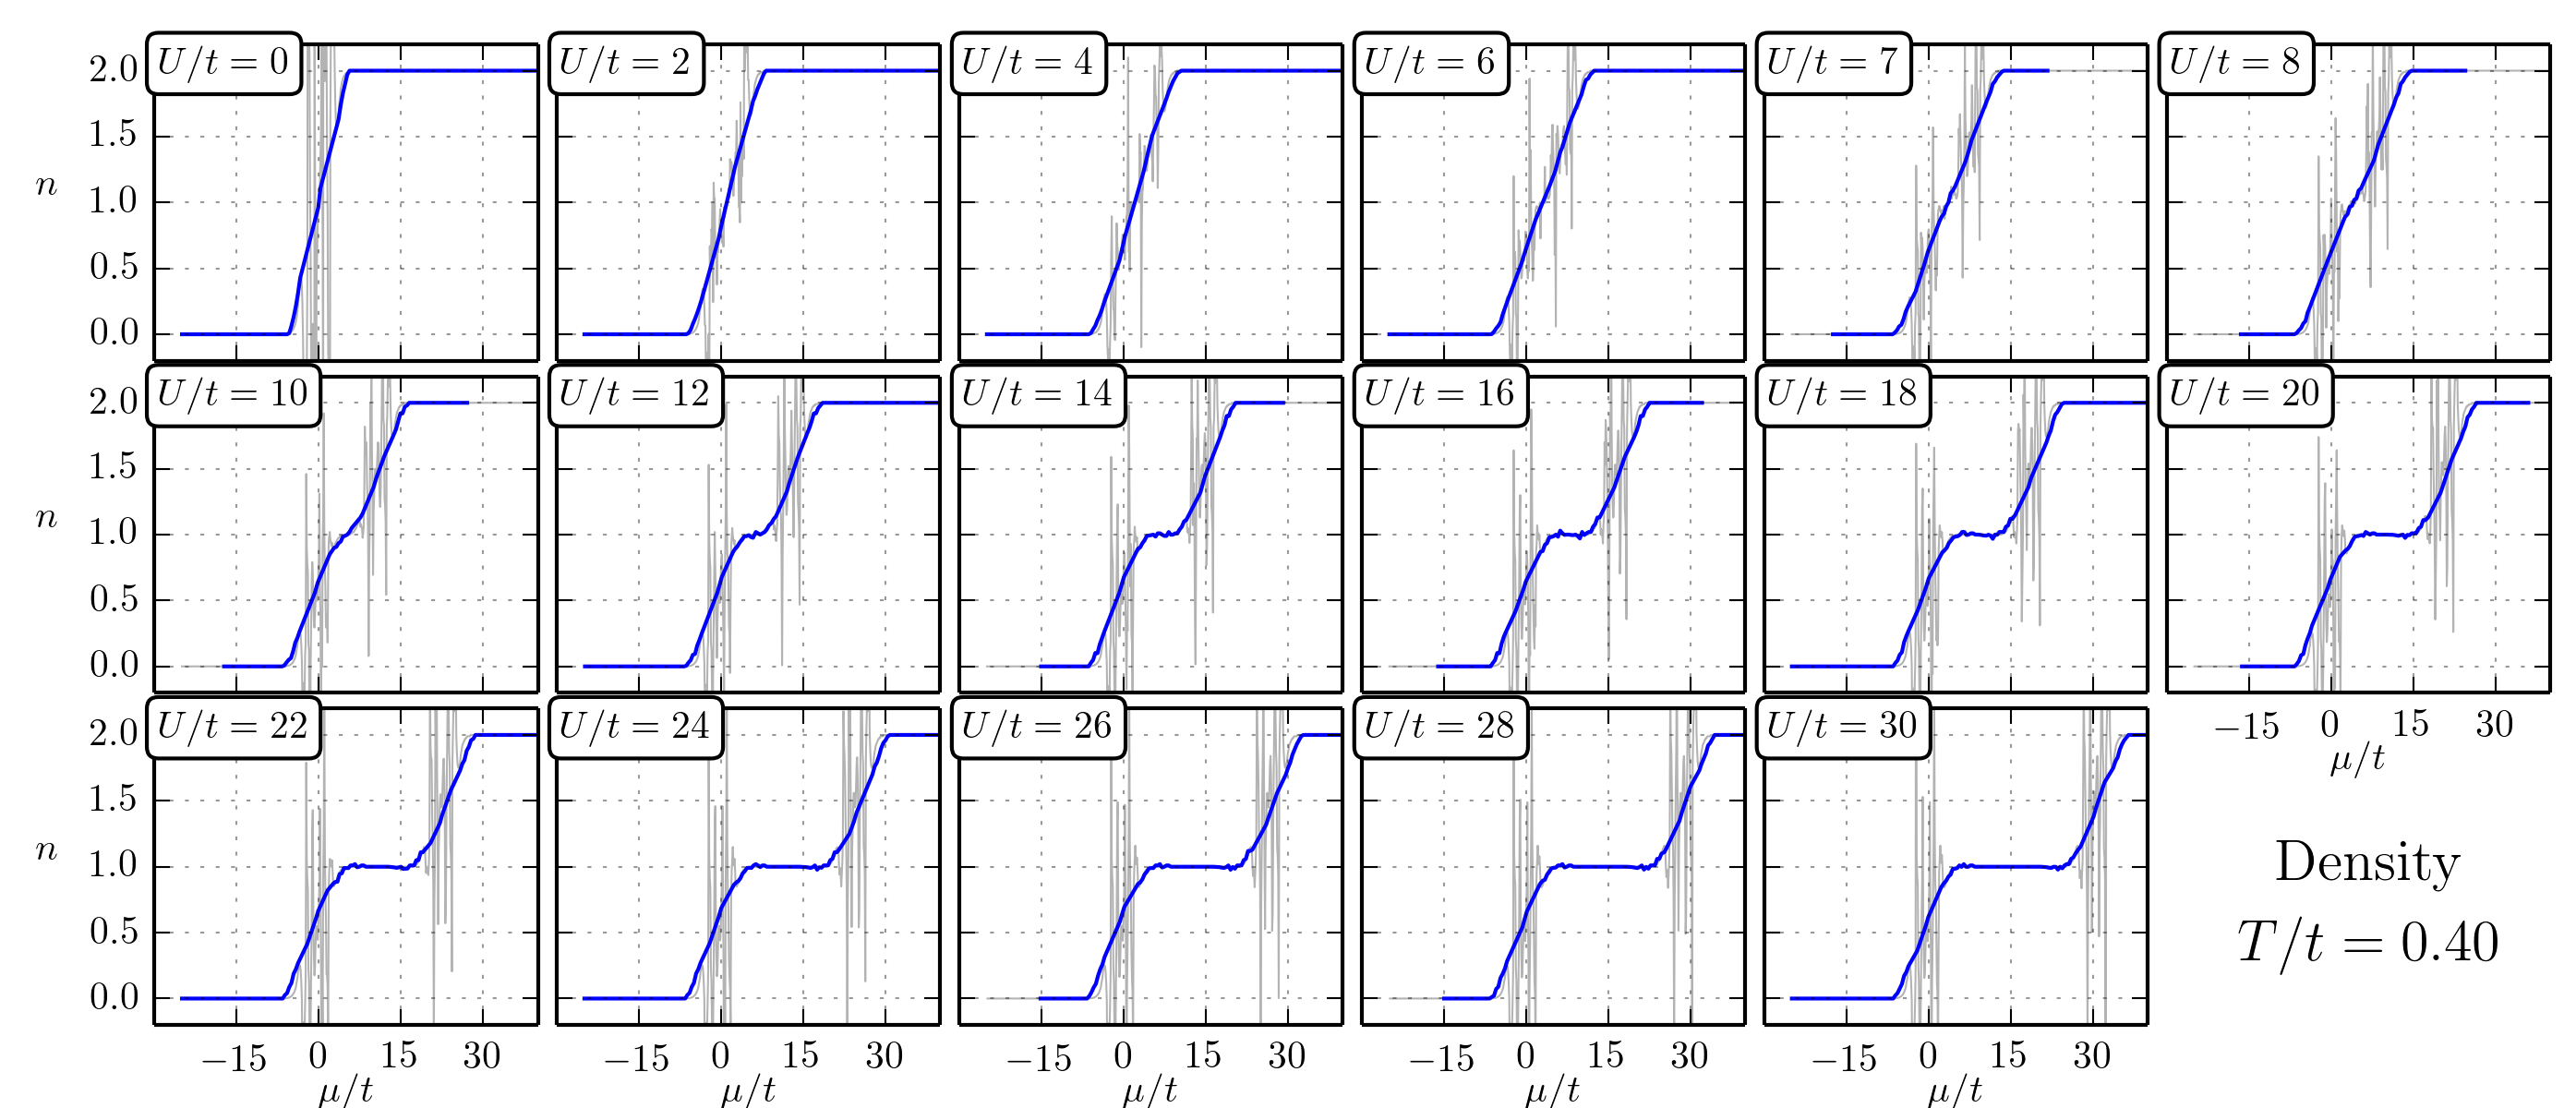
\includegraphics[width=1.0\textwidth]{../dataplots/NLCE_Final/density/T0_40.png}
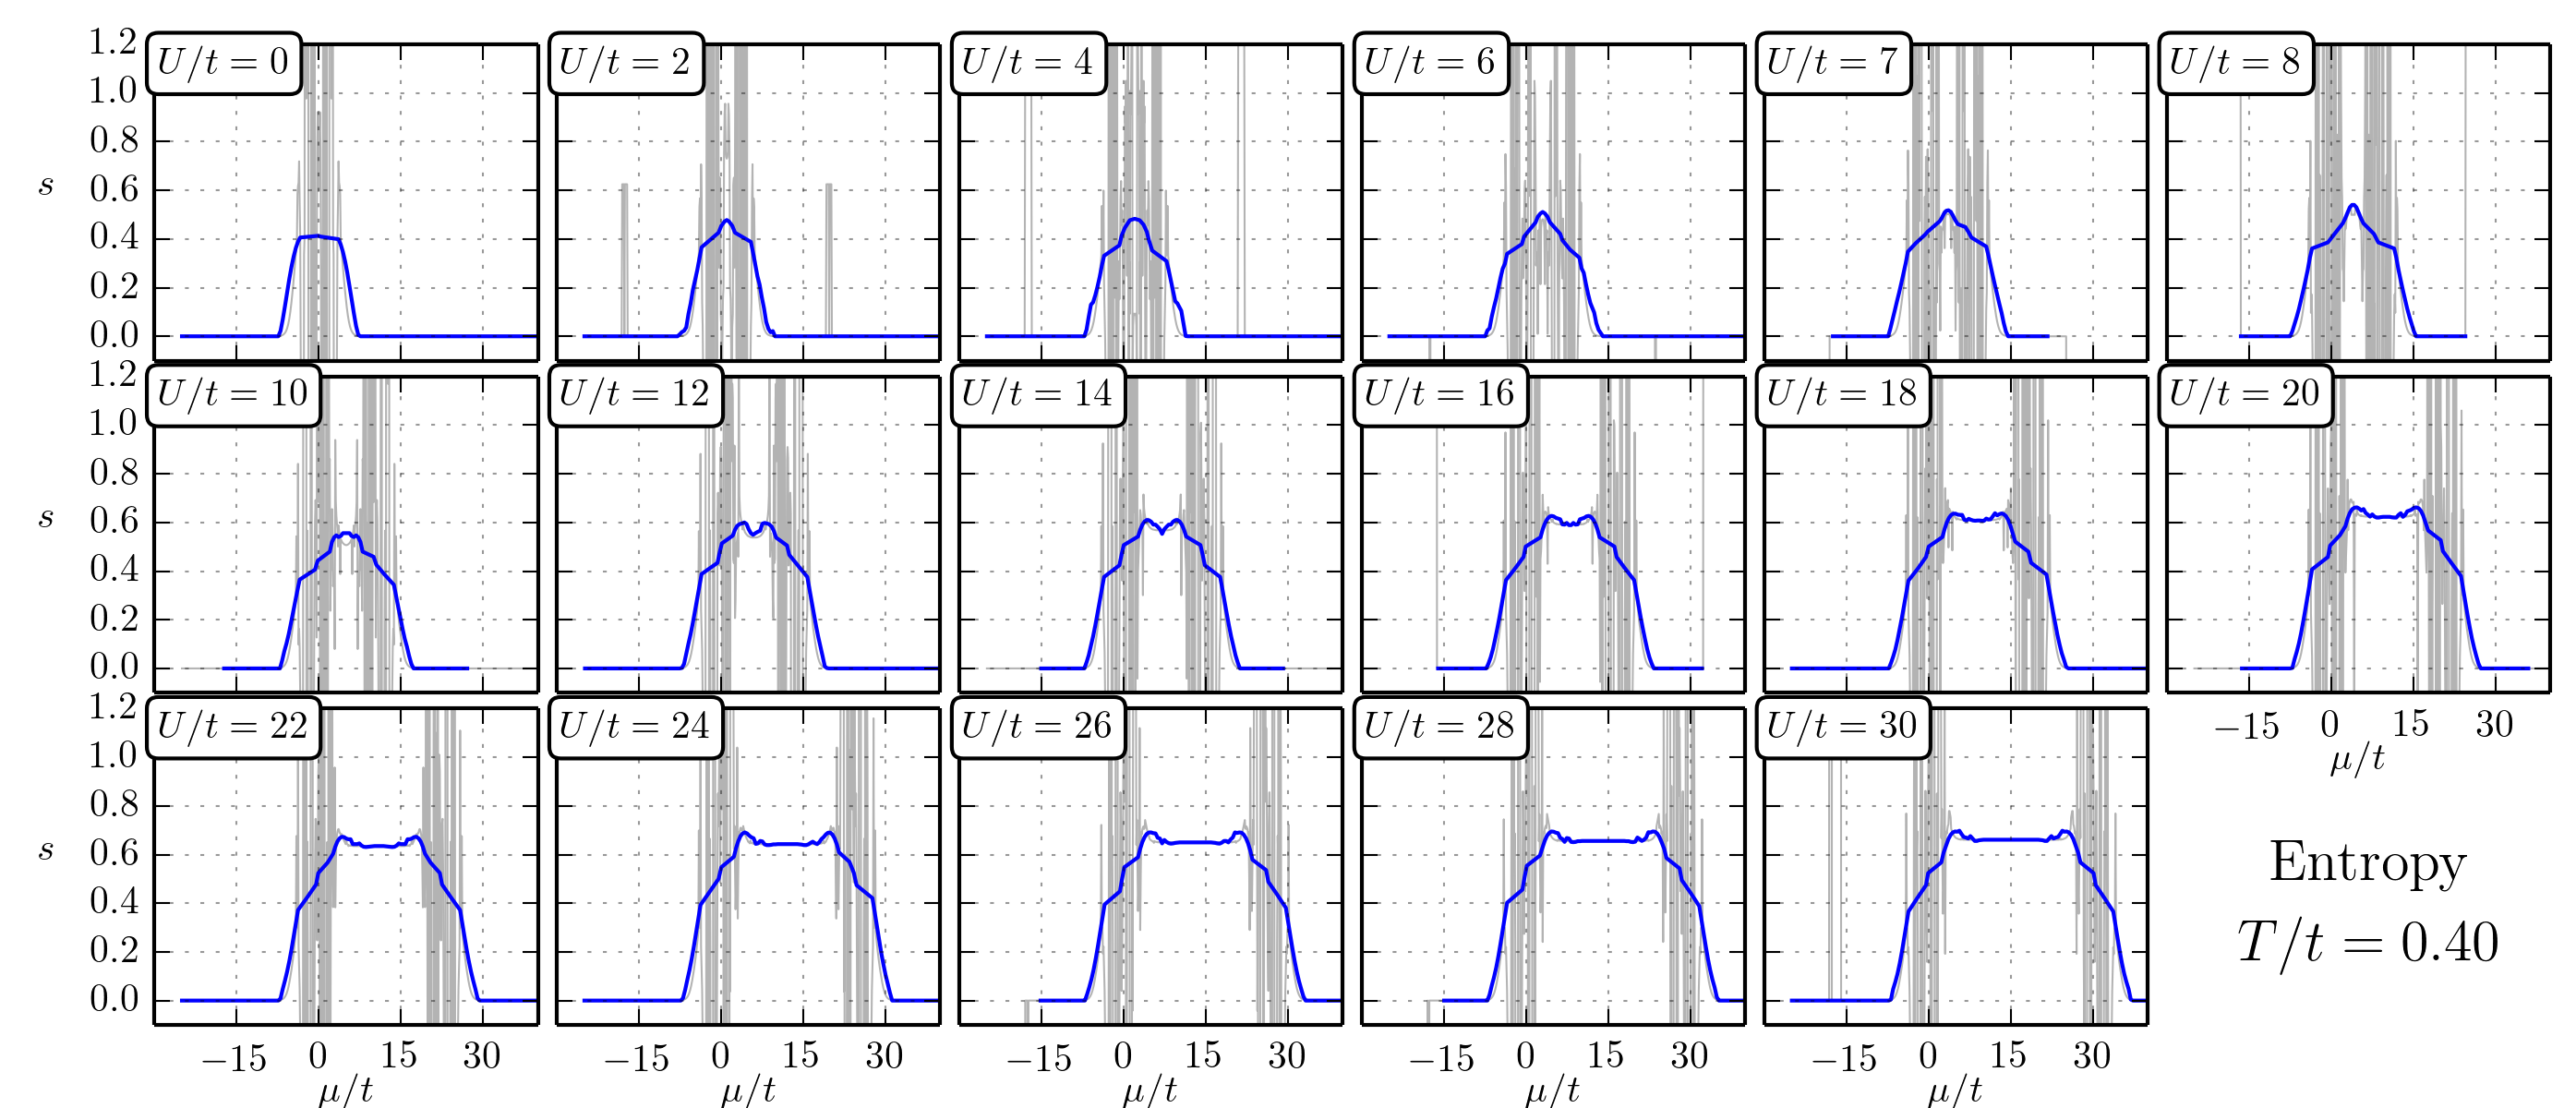
\includegraphics[width=1.0\textwidth]{../dataplots/NLCE_Final/entropy/T0_40.png}
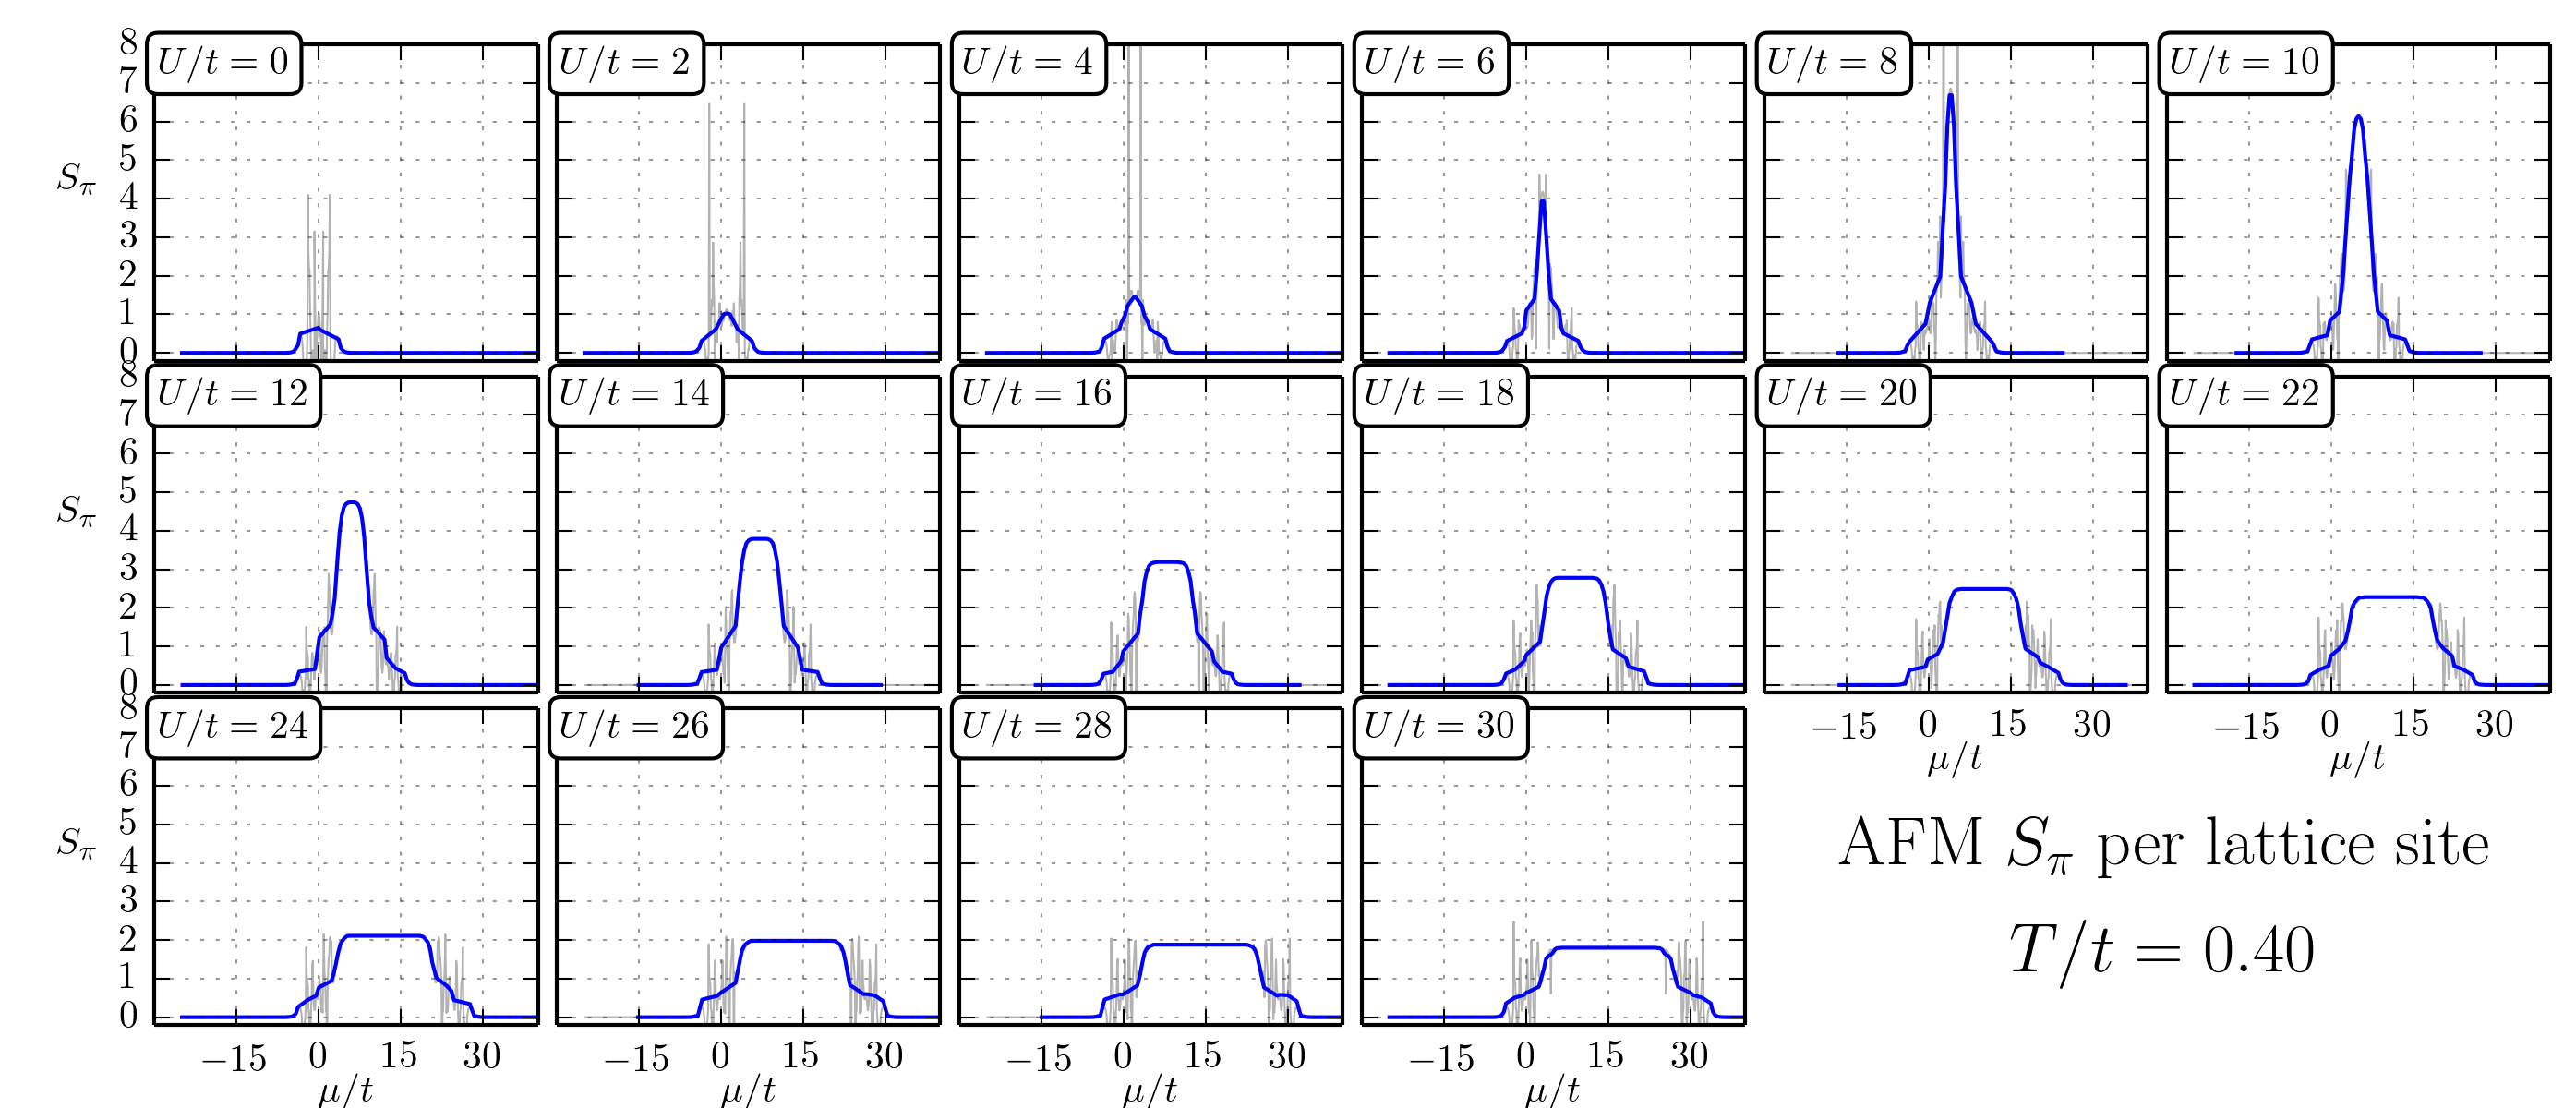
\includegraphics[width=1.0\textwidth]{../dataplots/NLCE_Final/spi/T0_40.png}
\caption{Lowest temperature data accessible to the NLCE by extrapolation,
$T/t=0.4$.  The original data provided by Ehsan is shown in gray and the data
after filtering is shown in blue.}
\label{fig:NLCE_T0.40}
\end{figure}

We can use the NLCE data to see that the density as a function of chemical
potential is pretty much frozen for $T/t<1.0$, see Fig.~\ref{fig:NLCEdens}.
The high temperature series expansion (HTSE) that I was using before to
calculate density profiles works down to about $T/t\approx 1.6$, so I was
unable to capture the ``Mottness'' of the density profile as we see it in the
experiment.
\begin{figure}
    \centering
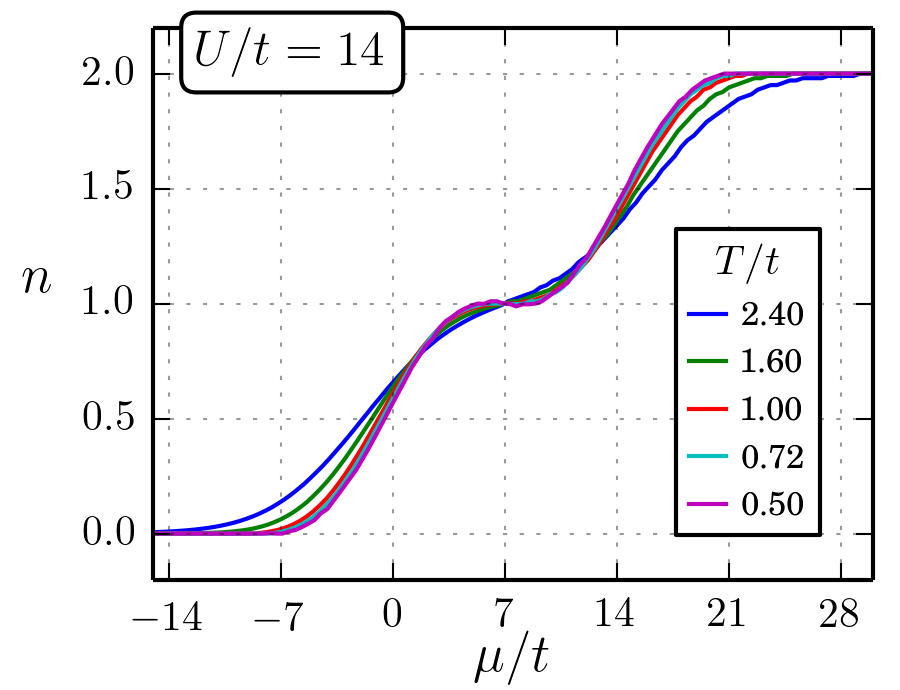
\includegraphics[width=0.6\textwidth]{../dataplots/NLCE_Final/U14_varyT.png}
\caption{NLCE data at $U/t=14$.  For $T/t \leq 1$ the density does not shown
much variation. }
\label{fig:NLCEdens}
\end{figure}


The data for $S_{\pi}/n$ provided by NLCE is shown in Fig.~\ref{fig:NLCESpin}.
Notice that to avoid errors when dividing by a small value of $n$ we have
decided to force all data to 1 for densities less than a density cutoff.  The
density cutoff is adjusted for each value of $U/t$.
\begin{figure}
    \centering
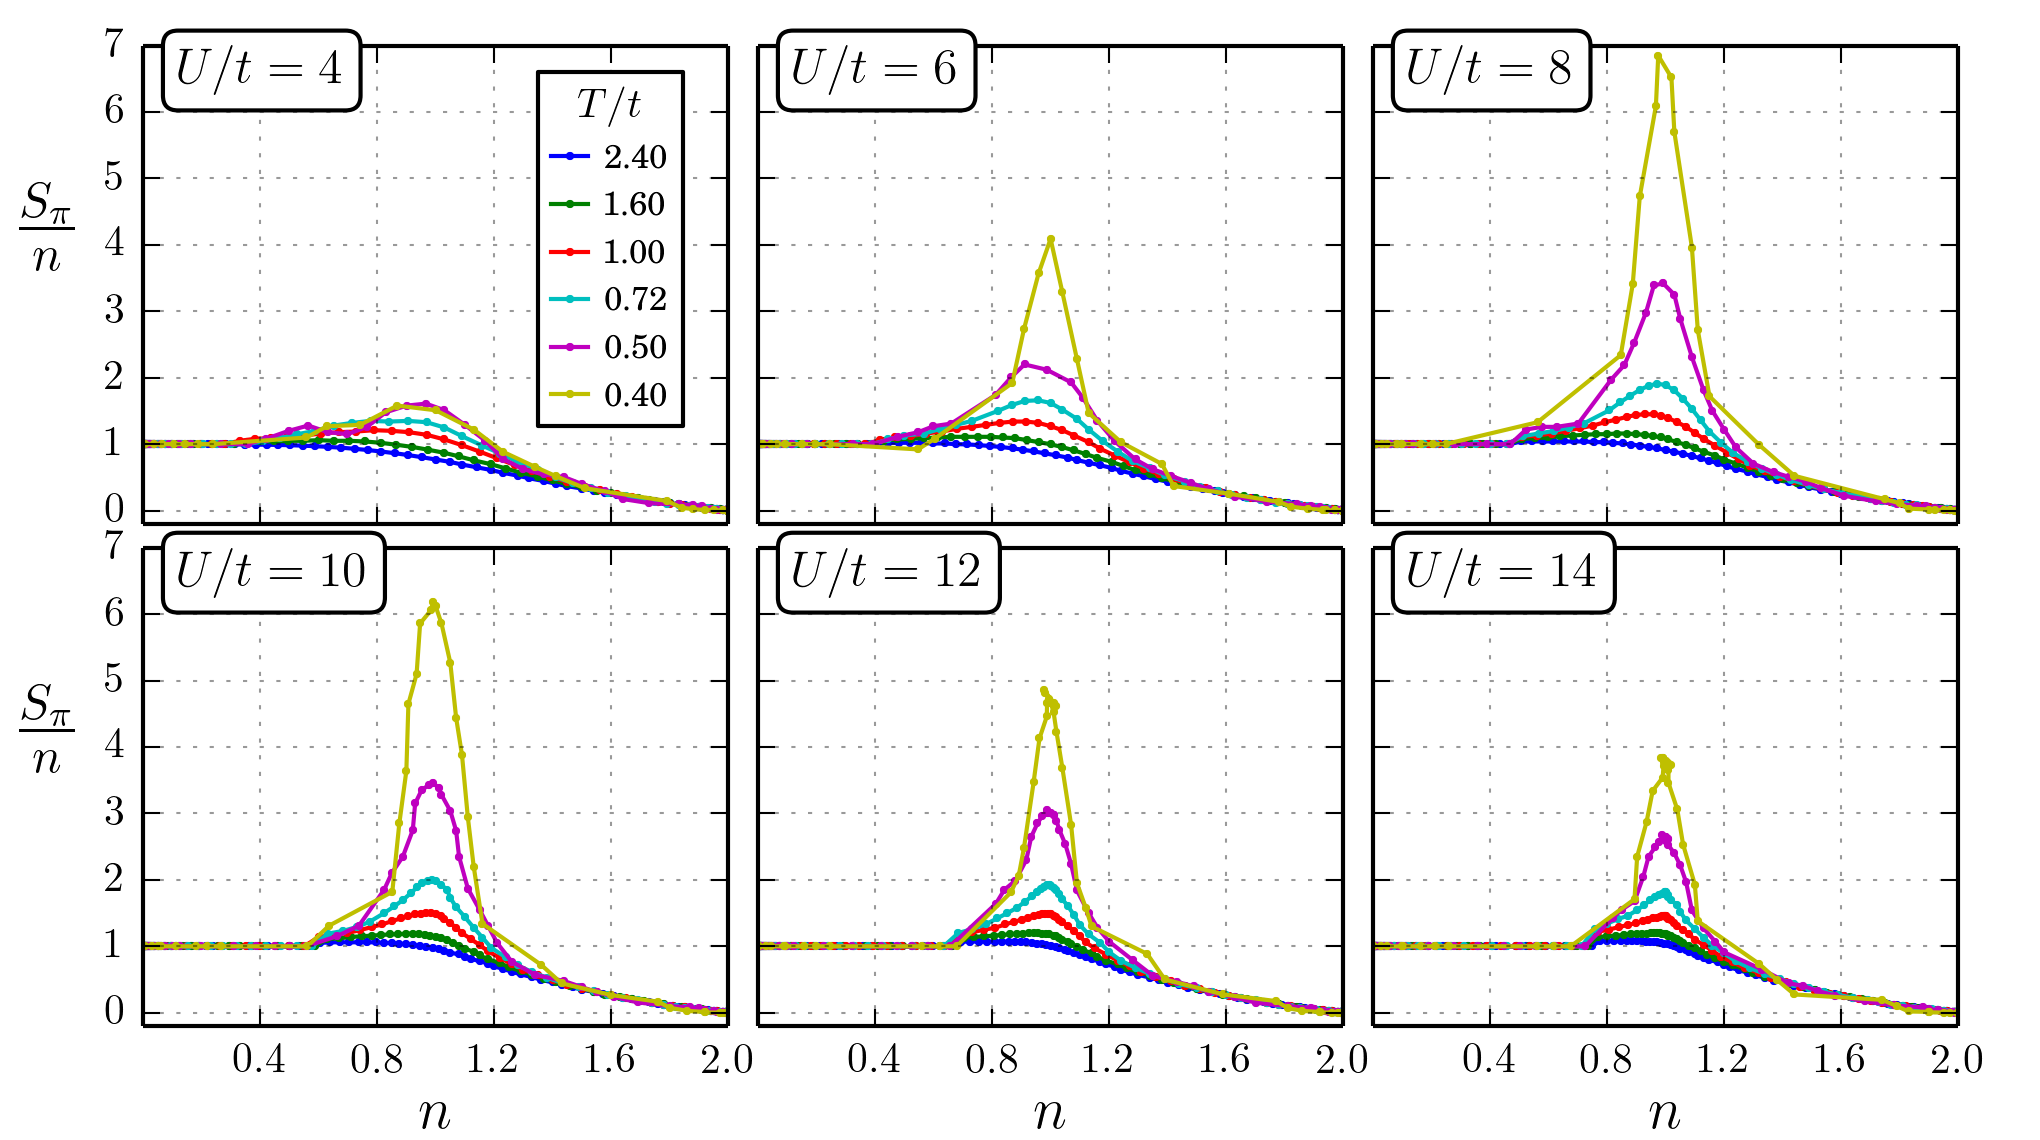
\includegraphics[width=\textwidth]{../dataplots/NLCE_Final/Spi_varyU_varyT.png}
\caption{NLCE $S_{\pi}/n$  data for various interactions and tempeatures.  }
\label{fig:NLCESpin}
\end{figure}

\section{ QMC data } 

The QMC data does not suffer from noise problems for small values of $T/t$,
however there is much less of it available.  Fig.~\ref{fig:QMCall} shows the
available $U/t$ and $T/t$ values.  The entropy and double occupancy, not shown
in the Figure are also available from Thereza's dataset,  as well as the
structure factor in the $\bv{\theta}$ direction. 
\begin{figure}
    \centering
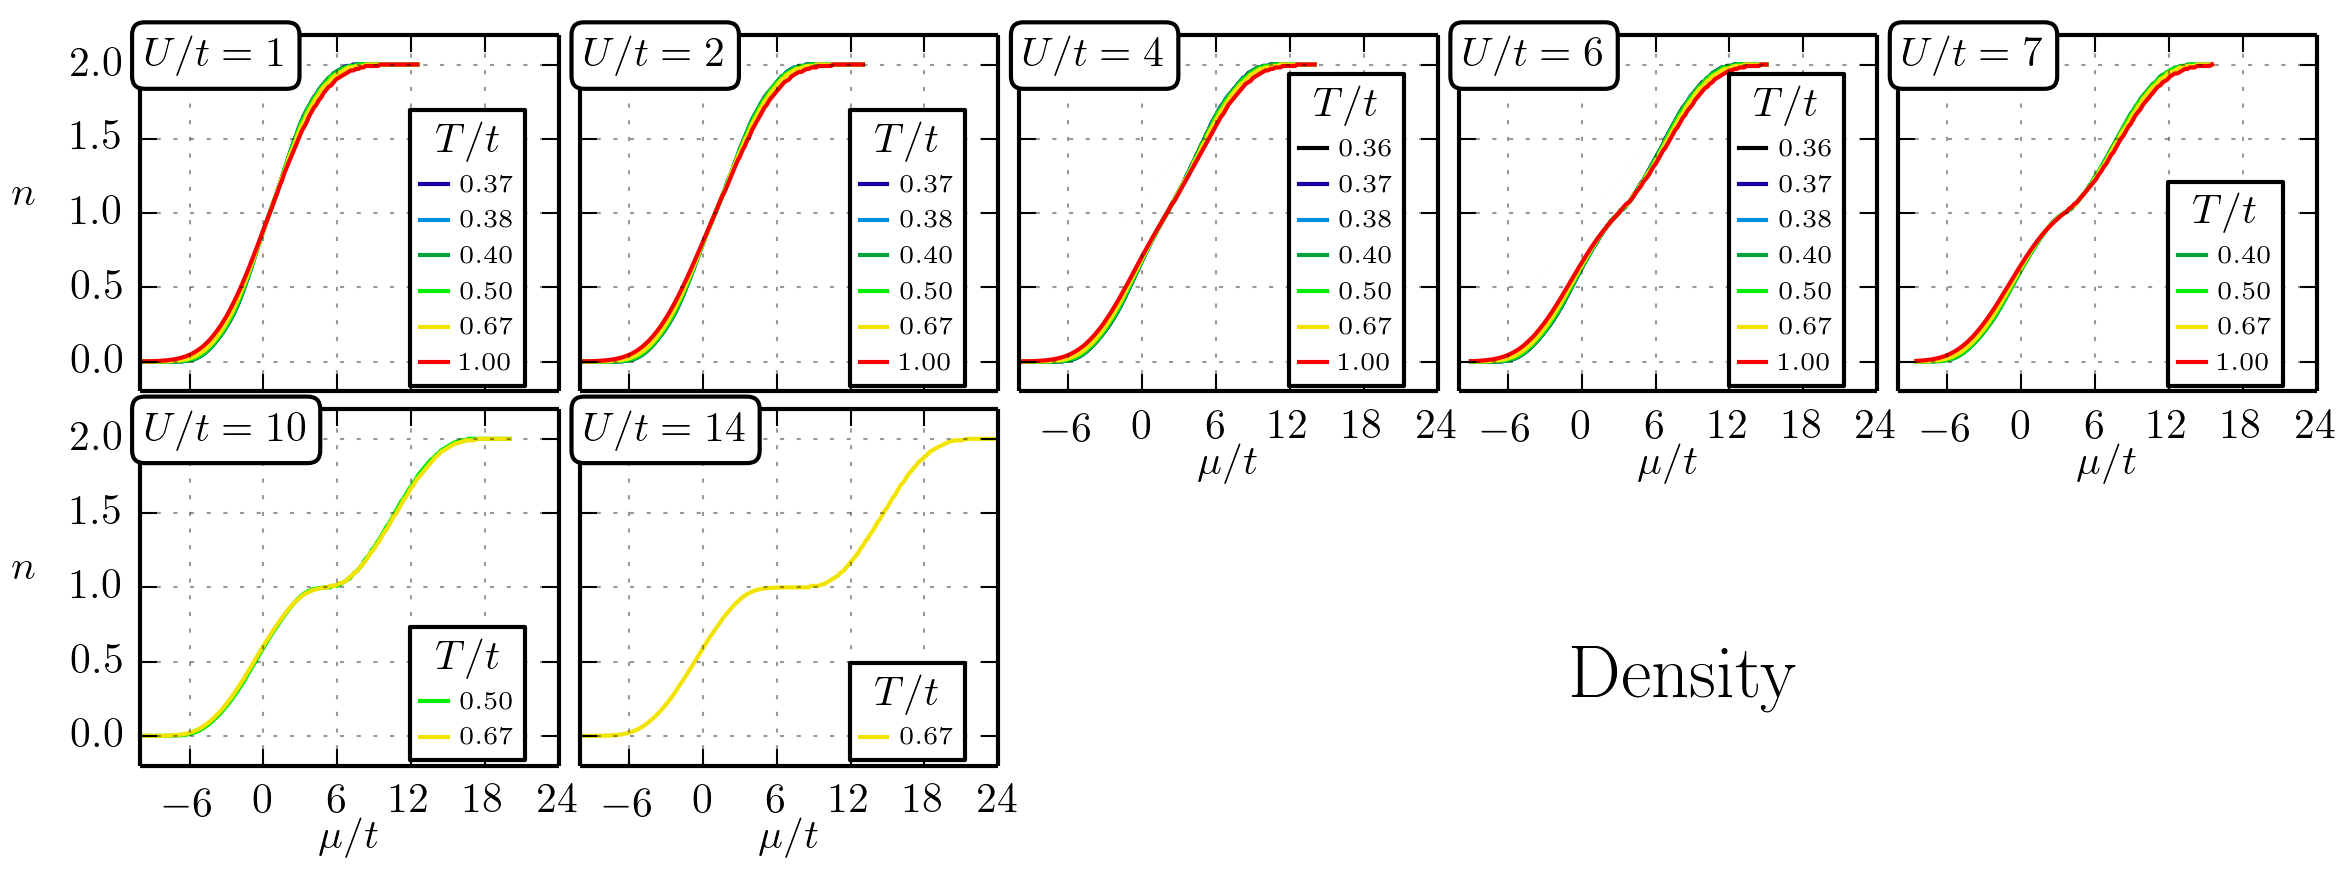
\includegraphics[width=\textwidth]{../dataplots/QMC_Final/density_All.png}
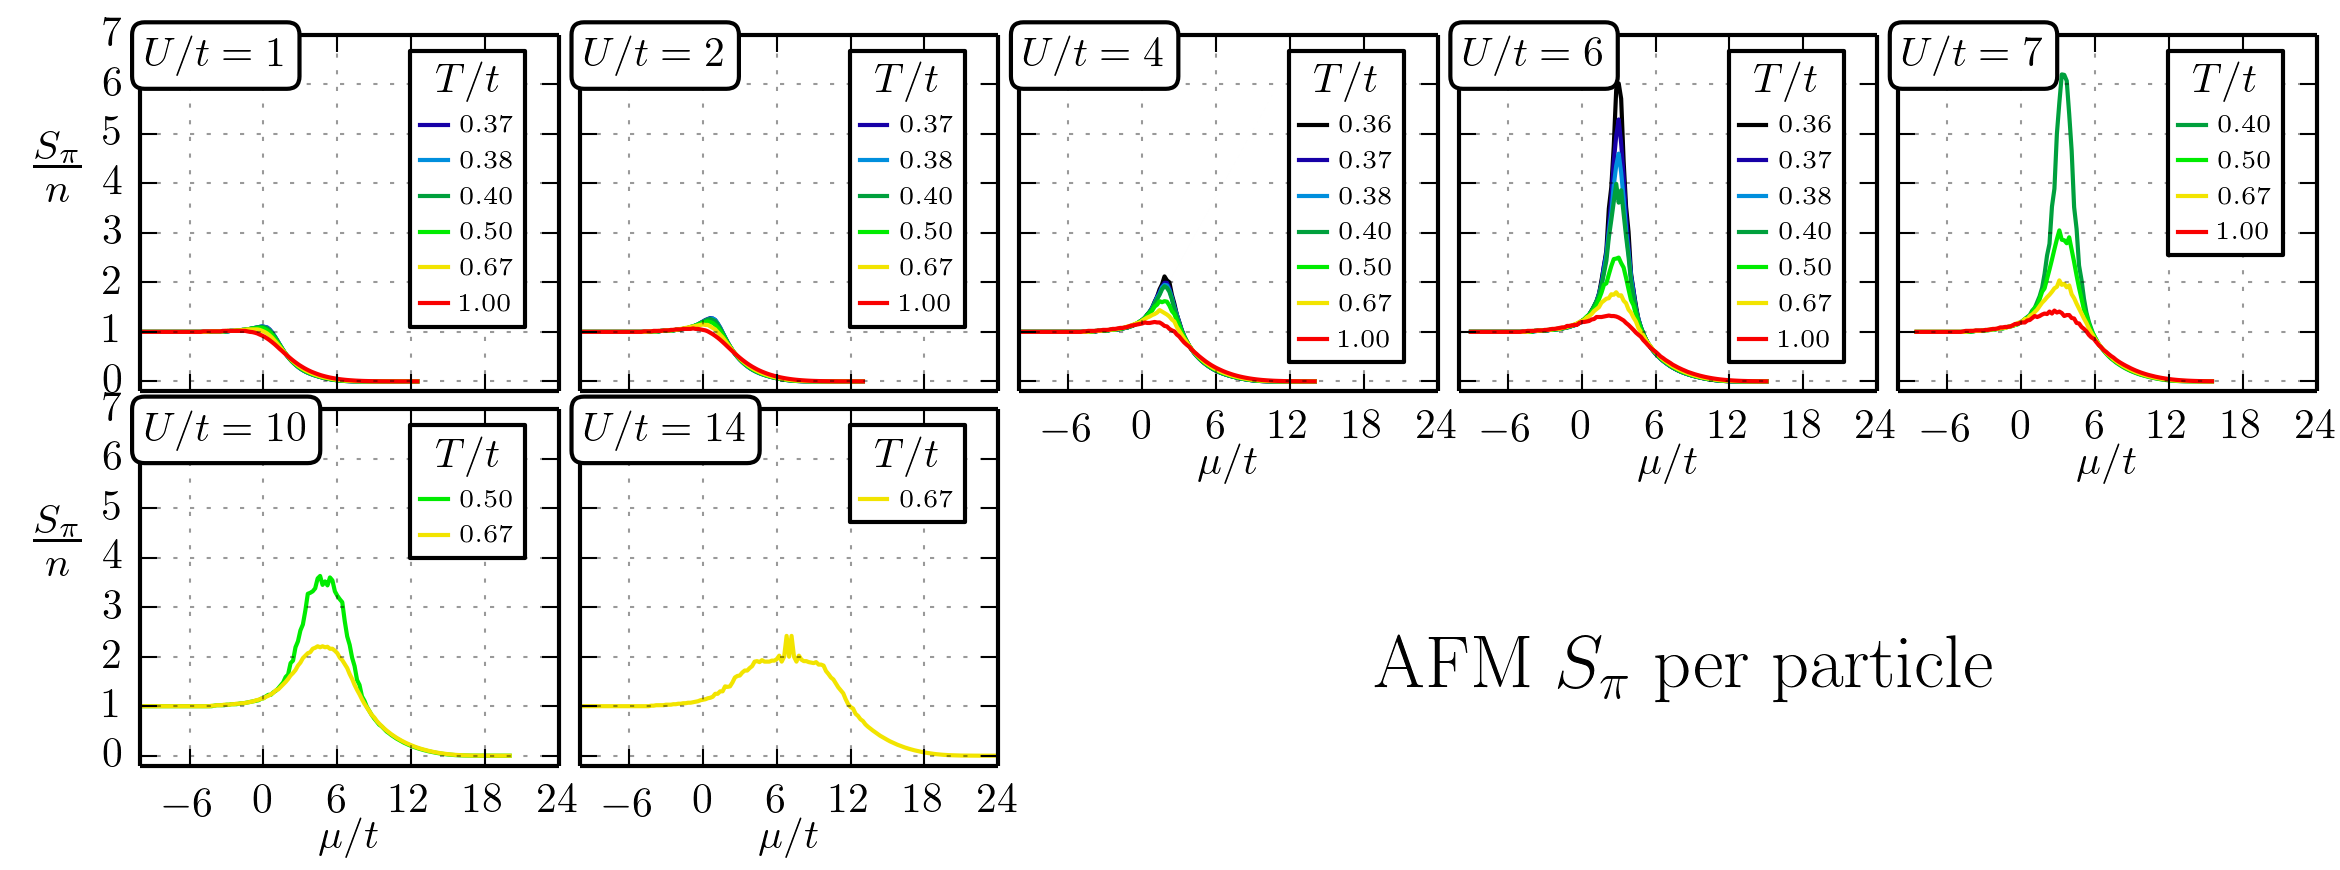
\includegraphics[width=\textwidth]{../dataplots/QMC_Final/spi_n_All.png}
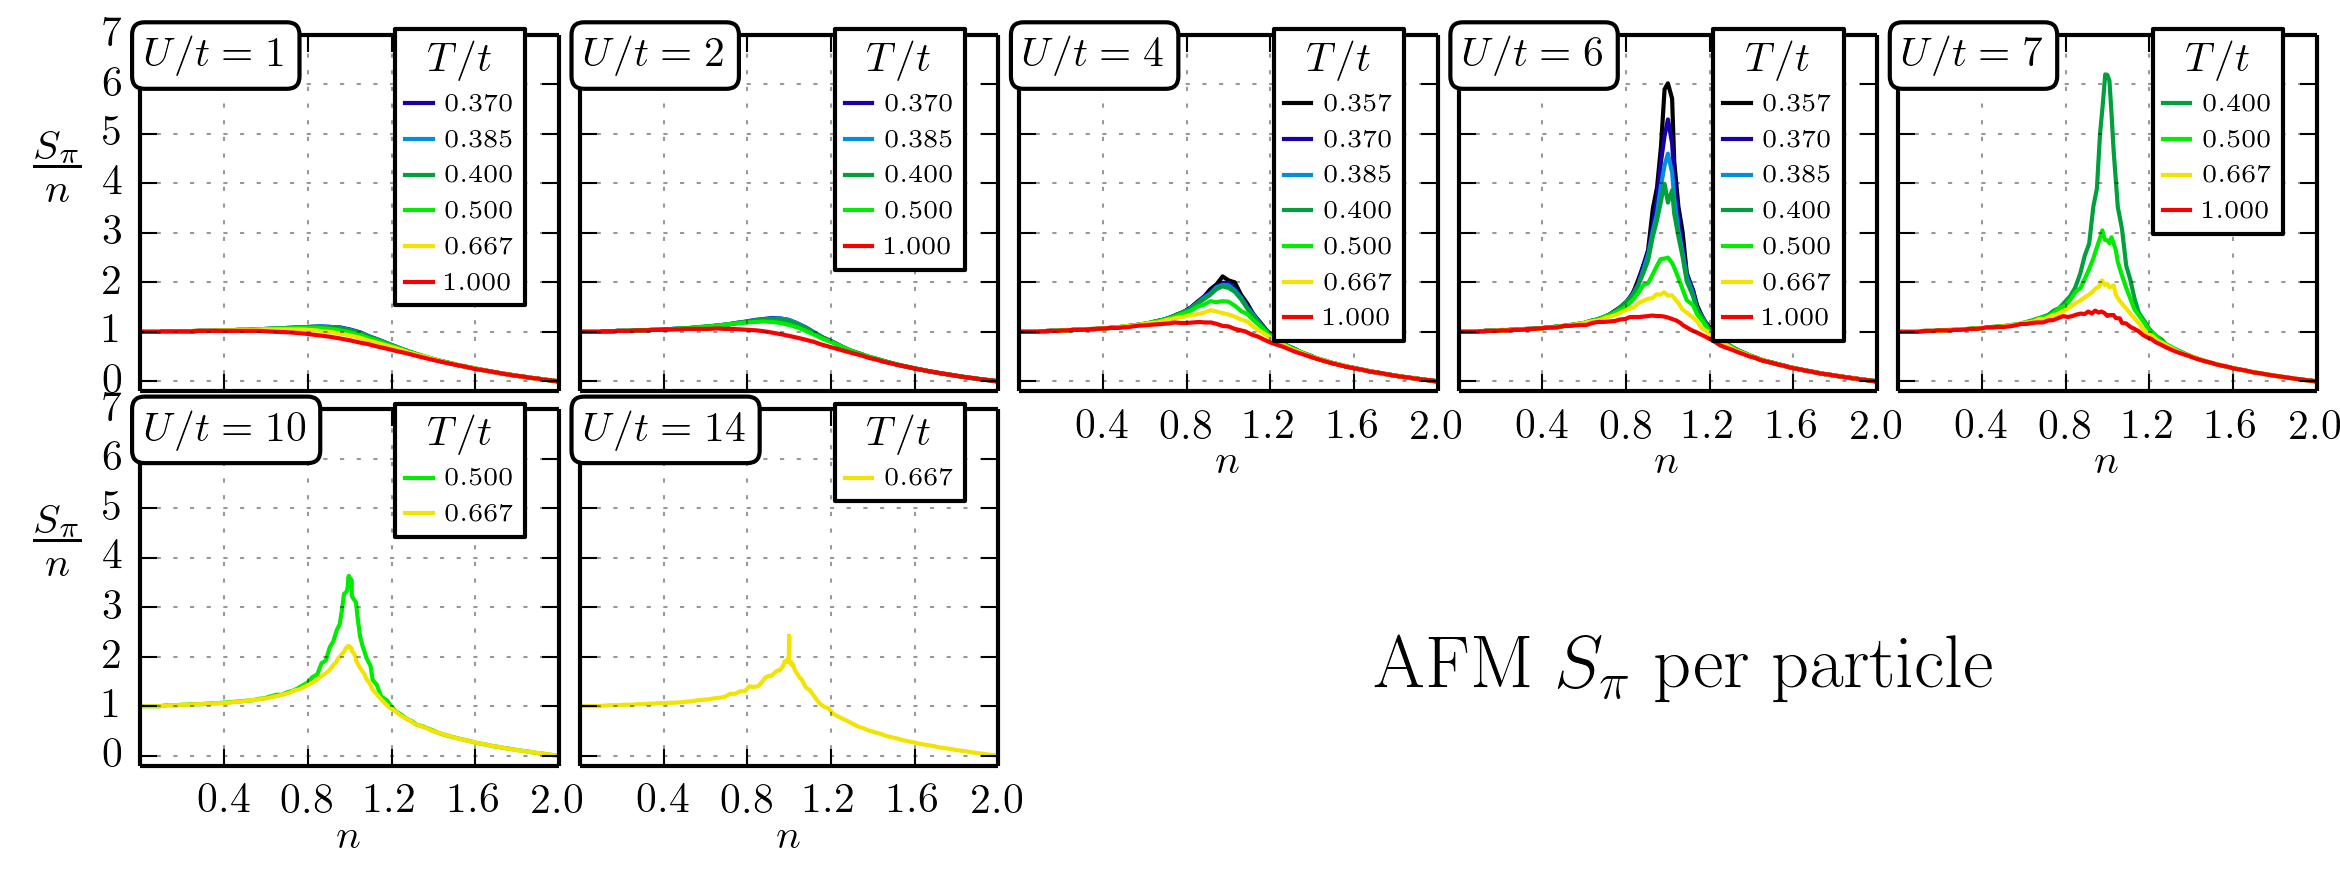
\includegraphics[width=\textwidth]{../dataplots/QMC_Final/spi_n_n_All.png}
\caption{All available QMC data.  Entropy, double occupancy and  $S_{\theta}/n$
not shown.  }
\label{fig:QMCall}
\end{figure}


\section{ NLCE data and QMC data comparison} 

In Fig.~\ref{fig:QMCvsNLCE} we show QMC and NLCE datasets side on the same
plot.  A direct comparison is possible at $U/t=6$, and then the QMC data at
$U/t=7$ is compared with NLCE at $U/t=8$ which reveals that the NLCE structure
factor is perhaps too broad as a function of $n$.   It is clear from this plots
that the density is frozen for $T/t < 1.0$ and that both QMC and NLCE have very
good agreement on the density. 
\begin{figure}
    \centering
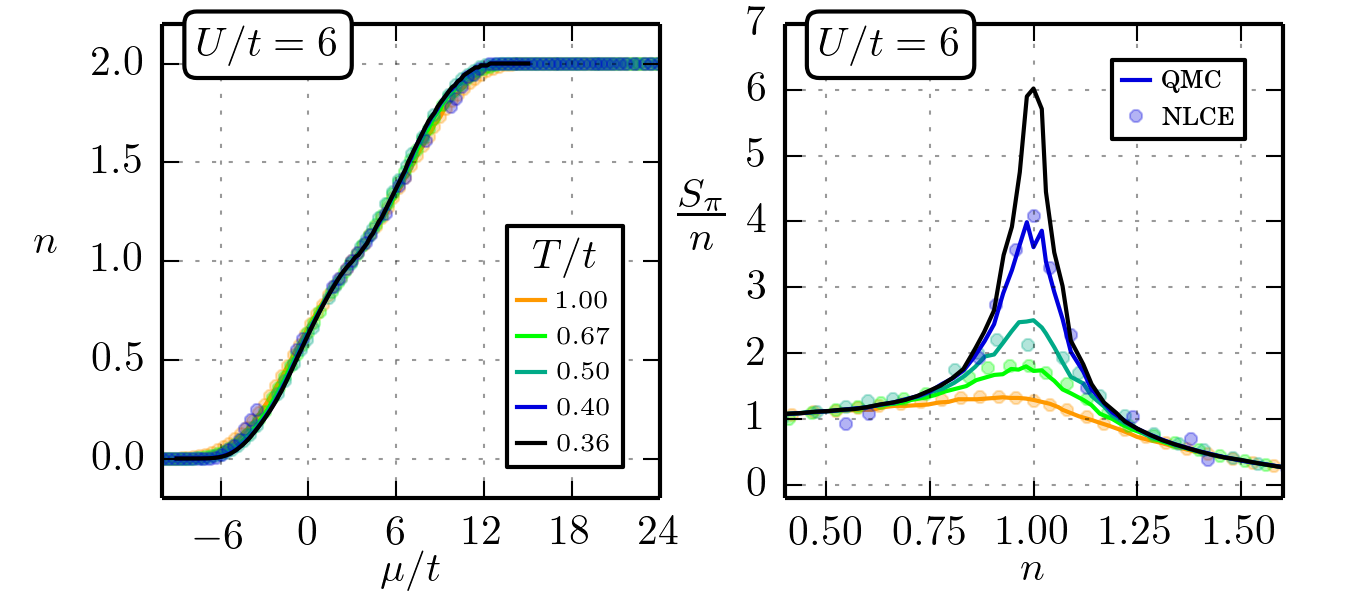
\includegraphics[width=\textwidth]{../dataplots/QMC_Final/QMC_NLCE_Compare_U06.png}
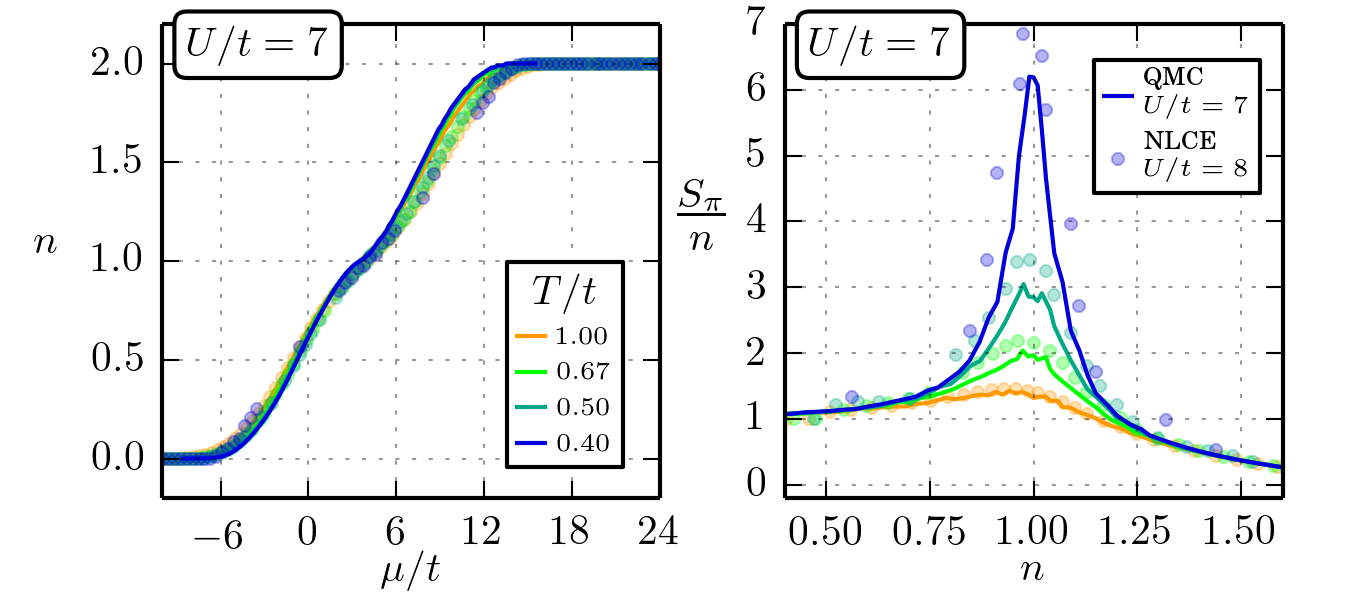
\includegraphics[width=\textwidth]{../dataplots/QMC_Final/QMC_NLCE_Compare_U07.png}
\caption{Comparison between QMC and NLCE data.  At $U/t=6$ both methods have
data available whereas the QMC data at $U/t=7$ is compared with the NLCE data
at $U/t=8$.}
\label{fig:QMCvsNLCE}
\end{figure}


\section{ Comparison of experimental data with theory } 

The way we will proceed is as follows:

\begin{enumerate}

  \item Set up a trap geometry based on our experimental calibration.  The trap
geometry determines the local chemical potential, the local $U/t$ and the local
$T/t$. 

  \item Use the NLCE data to calculate a density profile with the above
parameters.  The temperature used needs to be $T/t < 1.0$, since $n(\mu)$ is
frozen below this temperature, the obtained density profile is good for all
$T/t<1$. 

  \item Set a value of $[T/t]_{0}$, this is the local value of $T/t$ at the
center of the trap.  Use the local $n$ (from 2) along with the local $U/t$ and
$T/t$ to calculate the local $S_{\pi}/n$.   
 
  \item Integrate the local $S_{\pi}/n$ over the trap to obtain the bulk spin
structure factor $\bar{S}_{\pi}$. 

  \item Repeat 3 and 4 for different valus of $[T/t]_{0}$ until the resulting
$\bar{S}_{\pi}$ agrees with the experimental measurement. 
\end{enumerate}

From the discussion in the previous section we have established that the
density is very well characterized by either the NLCE or the QMC data.   On the
other hand, $S_{\pi}/n$ is not so good from NLCE at low temperatures and is not
availabe for many $U/t$ and $T/t$ from QMC.    For comparing with theory we
have put together a combined QMC + NLCE data set and for step 3 in the
prescription we interpolate linearly between the available points in the data
set in order to get $S_{\pi}/n$ at arbitrary values of $n$, $U/t$ and $T/t$.

\subsection{ LDA density profiles with NLCE data, variation with $T$}

In the experiment we varied the atom number to maximize the Bragg signal for a
given value of $[U/t]_{0}$.   The optimal atom number and the trap geometry
determine the global chemical potential to be used in the LDA to determine the
density profile.

To illustrate the effect of temperature on the density profile we show in
Fig.~\ref{fig:dens_varyT}  density profiles with $n=1$ at the center,
calculated for various values of $[T/t]_{0}$,  where $[T/t]_{0}$ is the local
value of $T/t$ at the center of the cloud.  The sample is assumed to be
isothermal so it has constant $T$ throughout, the local value of $t$ varies due
to the size of the lattice beams.
\begin{figure}
    \centering
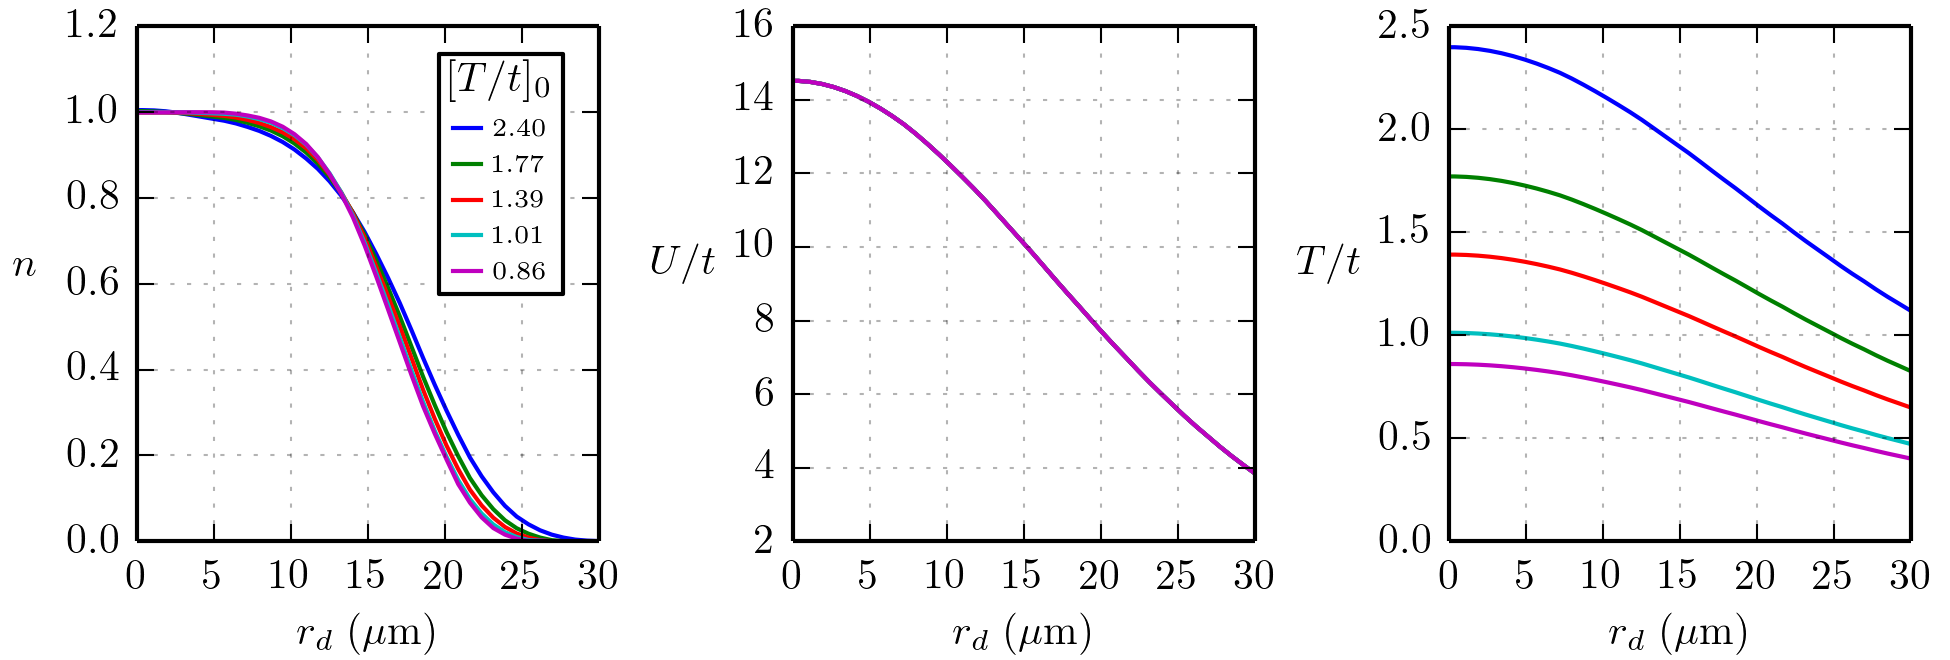
\includegraphics[width=\textwidth]{../dataplots/Basic00/density_varyT.png}
\caption{Density profiles with $n=1$ at the center for various values of
$[T/t]_{0}$. For $[T/t]_{0}<1$ the density profile changes very little with
temperature.  The right two panes show the spatial variation of $U/t$ and $T/t$
across the sample, illustrating the degree of inhomogeneity in the system. }
\label{fig:dens_varyT}
\end{figure}
As expected we se that for $[T/t]_{0} < 1 $ the density profile does not change
very much, which validates our approach of calculating the density profile only
once with NLCE.  See step 2 in the prescription outlined above.

 


 
 

 
\bibliographystyle{osa} \bibliography{latt_evap}

\end{document}




